%%%%%%%%%%%%%%%%%%%%%%%%%%%%%%%%%%%%%
%                                   %
% Compile with XeLaTeX and biber    %
%                                   %
% Questions or comments:            %
%                                   %
% joshua dot mcneill at uga dot edu %
%                                   %
%%%%%%%%%%%%%%%%%%%%%%%%%%%%%%%%%%%%%

\documentclass{beamer}
  % Read in standard preamble (cosmetic stuff)
  %%%%%%%%%%%%%%%%%%%%%%%%%%%%%%%%%%%%%%%%%%%%%%%%%%%%%%%%%%%%%%%%
% This is a standard preamble used in for all slide documents. %
% It basically contains cosmetic settings.                     %
%                                                              %
% Joshua McNeill                                               %
% joshua dot mcneill at uga dot edu                            %
%%%%%%%%%%%%%%%%%%%%%%%%%%%%%%%%%%%%%%%%%%%%%%%%%%%%%%%%%%%%%%%%

% Beamer settings
% \usetheme{Berkeley}
\usetheme{CambridgeUS}
% \usecolortheme{dove}
% \usecolortheme{rose}
\usecolortheme{seagull}
\usefonttheme{professionalfonts}
\usefonttheme{serif}
\setbeamertemplate{bibliography item}{}

% Packages and settings
\usepackage{fontspec}
  \setmainfont{Charis SIL}
\usepackage{hyperref}
  \hypersetup{colorlinks=true,
              allcolors=blue}
\usepackage{graphicx}
  \graphicspath{{../../figures/}}
\usepackage[normalem]{ulem}
\usepackage{enumerate}

% Document information
\author{M. McNeill}
\title[FREN2001]{Français 2001}
\institute{\url{joshua.mcneill@uga.edu}}
\date{}

%% Custom commands
% Lexical items
\newcommand{\lexi}[1]{\textit{#1}}
% Gloss
\newcommand{\gloss}[1]{`#1'}
\newcommand{\tinygloss}[1]{{\tiny`#1'}}
% Orthographic representations
\newcommand{\orth}[1]{$\langle$#1$\rangle$}
% Utterances (pragmatics)
\newcommand{\uttr}[1]{`#1'}
% Sentences (pragmatics)
\newcommand{\sent}[1]{\textit{#1}}
% Base dir for definitions
\newcommand{\defs}{../definitions}


  % Packages and settings

  % Document information
  \subtitle[Nombres et adjectifs]{Les nombres et les adjectifs}

\begin{document}
  % Read in the standard intro slides (title page and table of contents)
  \begin{frame}
    \titlepage
    \tiny{Office: % Basically a variable for office hours location
Gilbert 121\\
          Office hours: % Basically a variable for office hours
 lundi, mercredi, vendredi 10:10--11:10
}
  \end{frame}

  \begin{frame}{Annonces}
    \begin{itemize}
      \item No class Monday (Labor Day)!
    \end{itemize}
  \end{frame}

  \begin{frame}{Quel âge?}
    \begin{center}
      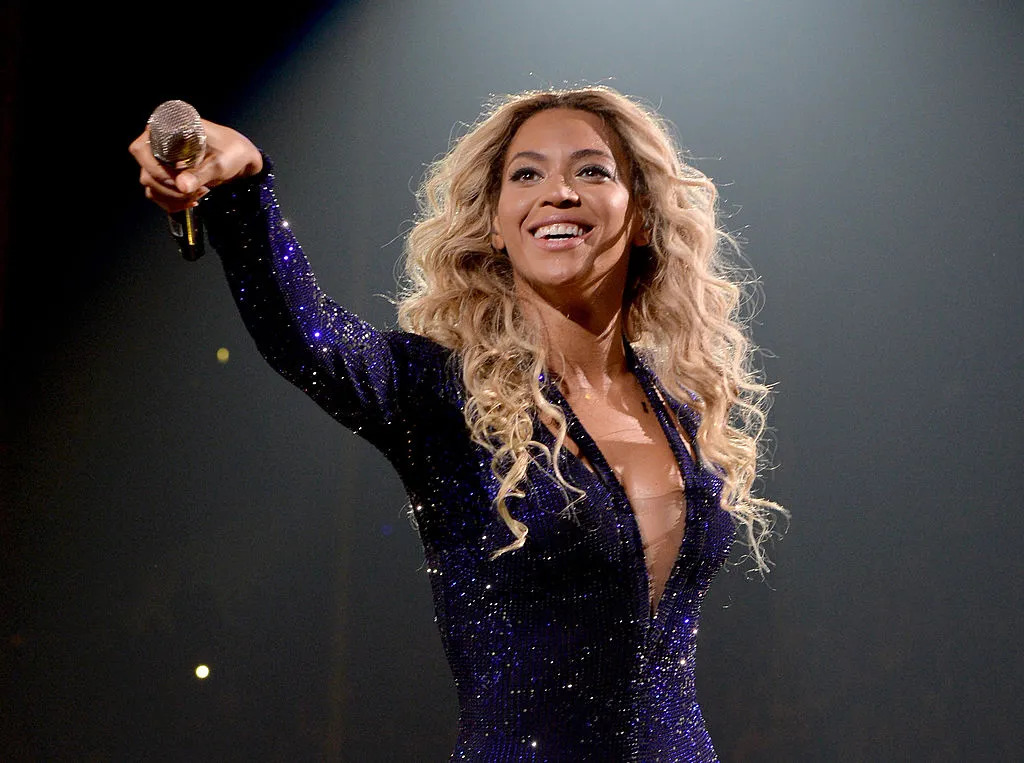
\includegraphics[scale=0.2]{beyonce.jpg}

      Elle a quel âge? \underline{\uncover<2->{Elle a 40 ans.}}
    \end{center}
  \end{frame}

  \begin{frame}{Quel âge?}
    \begin{center}
      
\includegraphics[scale=0.35]{emmanuel_macron.jpg}

      Il a quel âge? \underline{\uncover<2->{Il a 44 ans.}}
    \end{center}
  \end{frame}

  \begin{frame}{Quel âge?}
    \begin{center}
      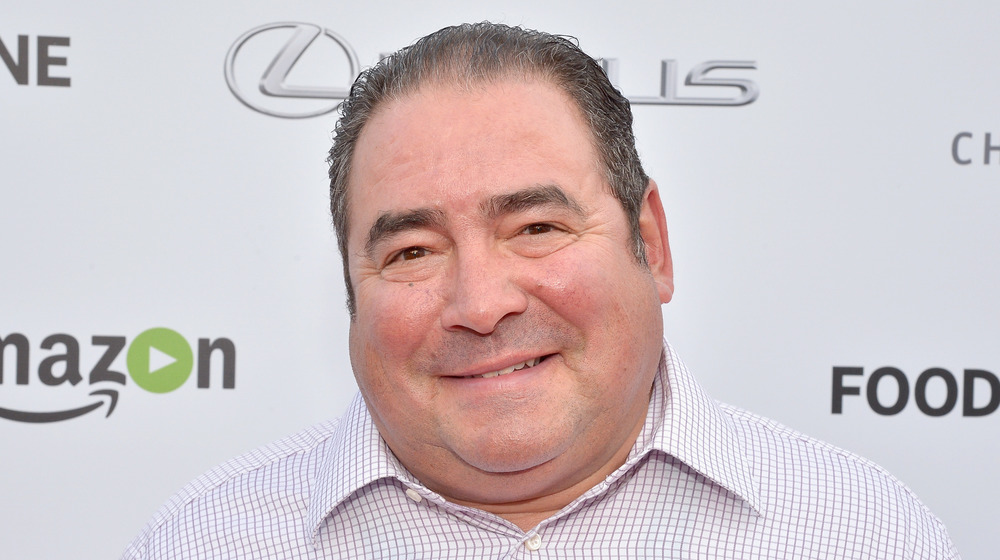
\includegraphics{emeril_lagasse.jpg}

      Il a quel âge? \underline{\uncover<2->{Il a 62 ans.}}
    \end{center}
  \end{frame}

  \begin{frame}{Quel âge?}
    \begin{center}
      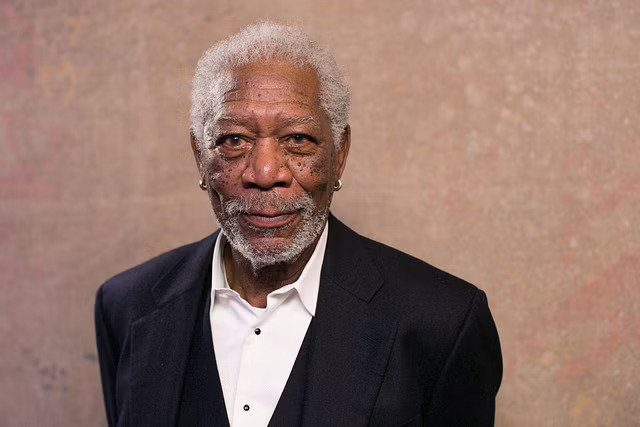
\includegraphics[scale=0.35]{morgan_freeman.jpg}

      Il a quel âge? \underline{\uncover<2->{Il a 85 ans.}}
    \end{center}
  \end{frame}

  \begin{frame}{Quel âge?}
    \begin{center}
      
\includegraphics[scale=0.45]{lea_seydoux.jpg}

      Elle a quel âge? \underline{\uncover<2->{Elle a 37 ans.}}
    \end{center}
  \end{frame}

  \begin{frame}{Quel âge?}
    \begin{center}
      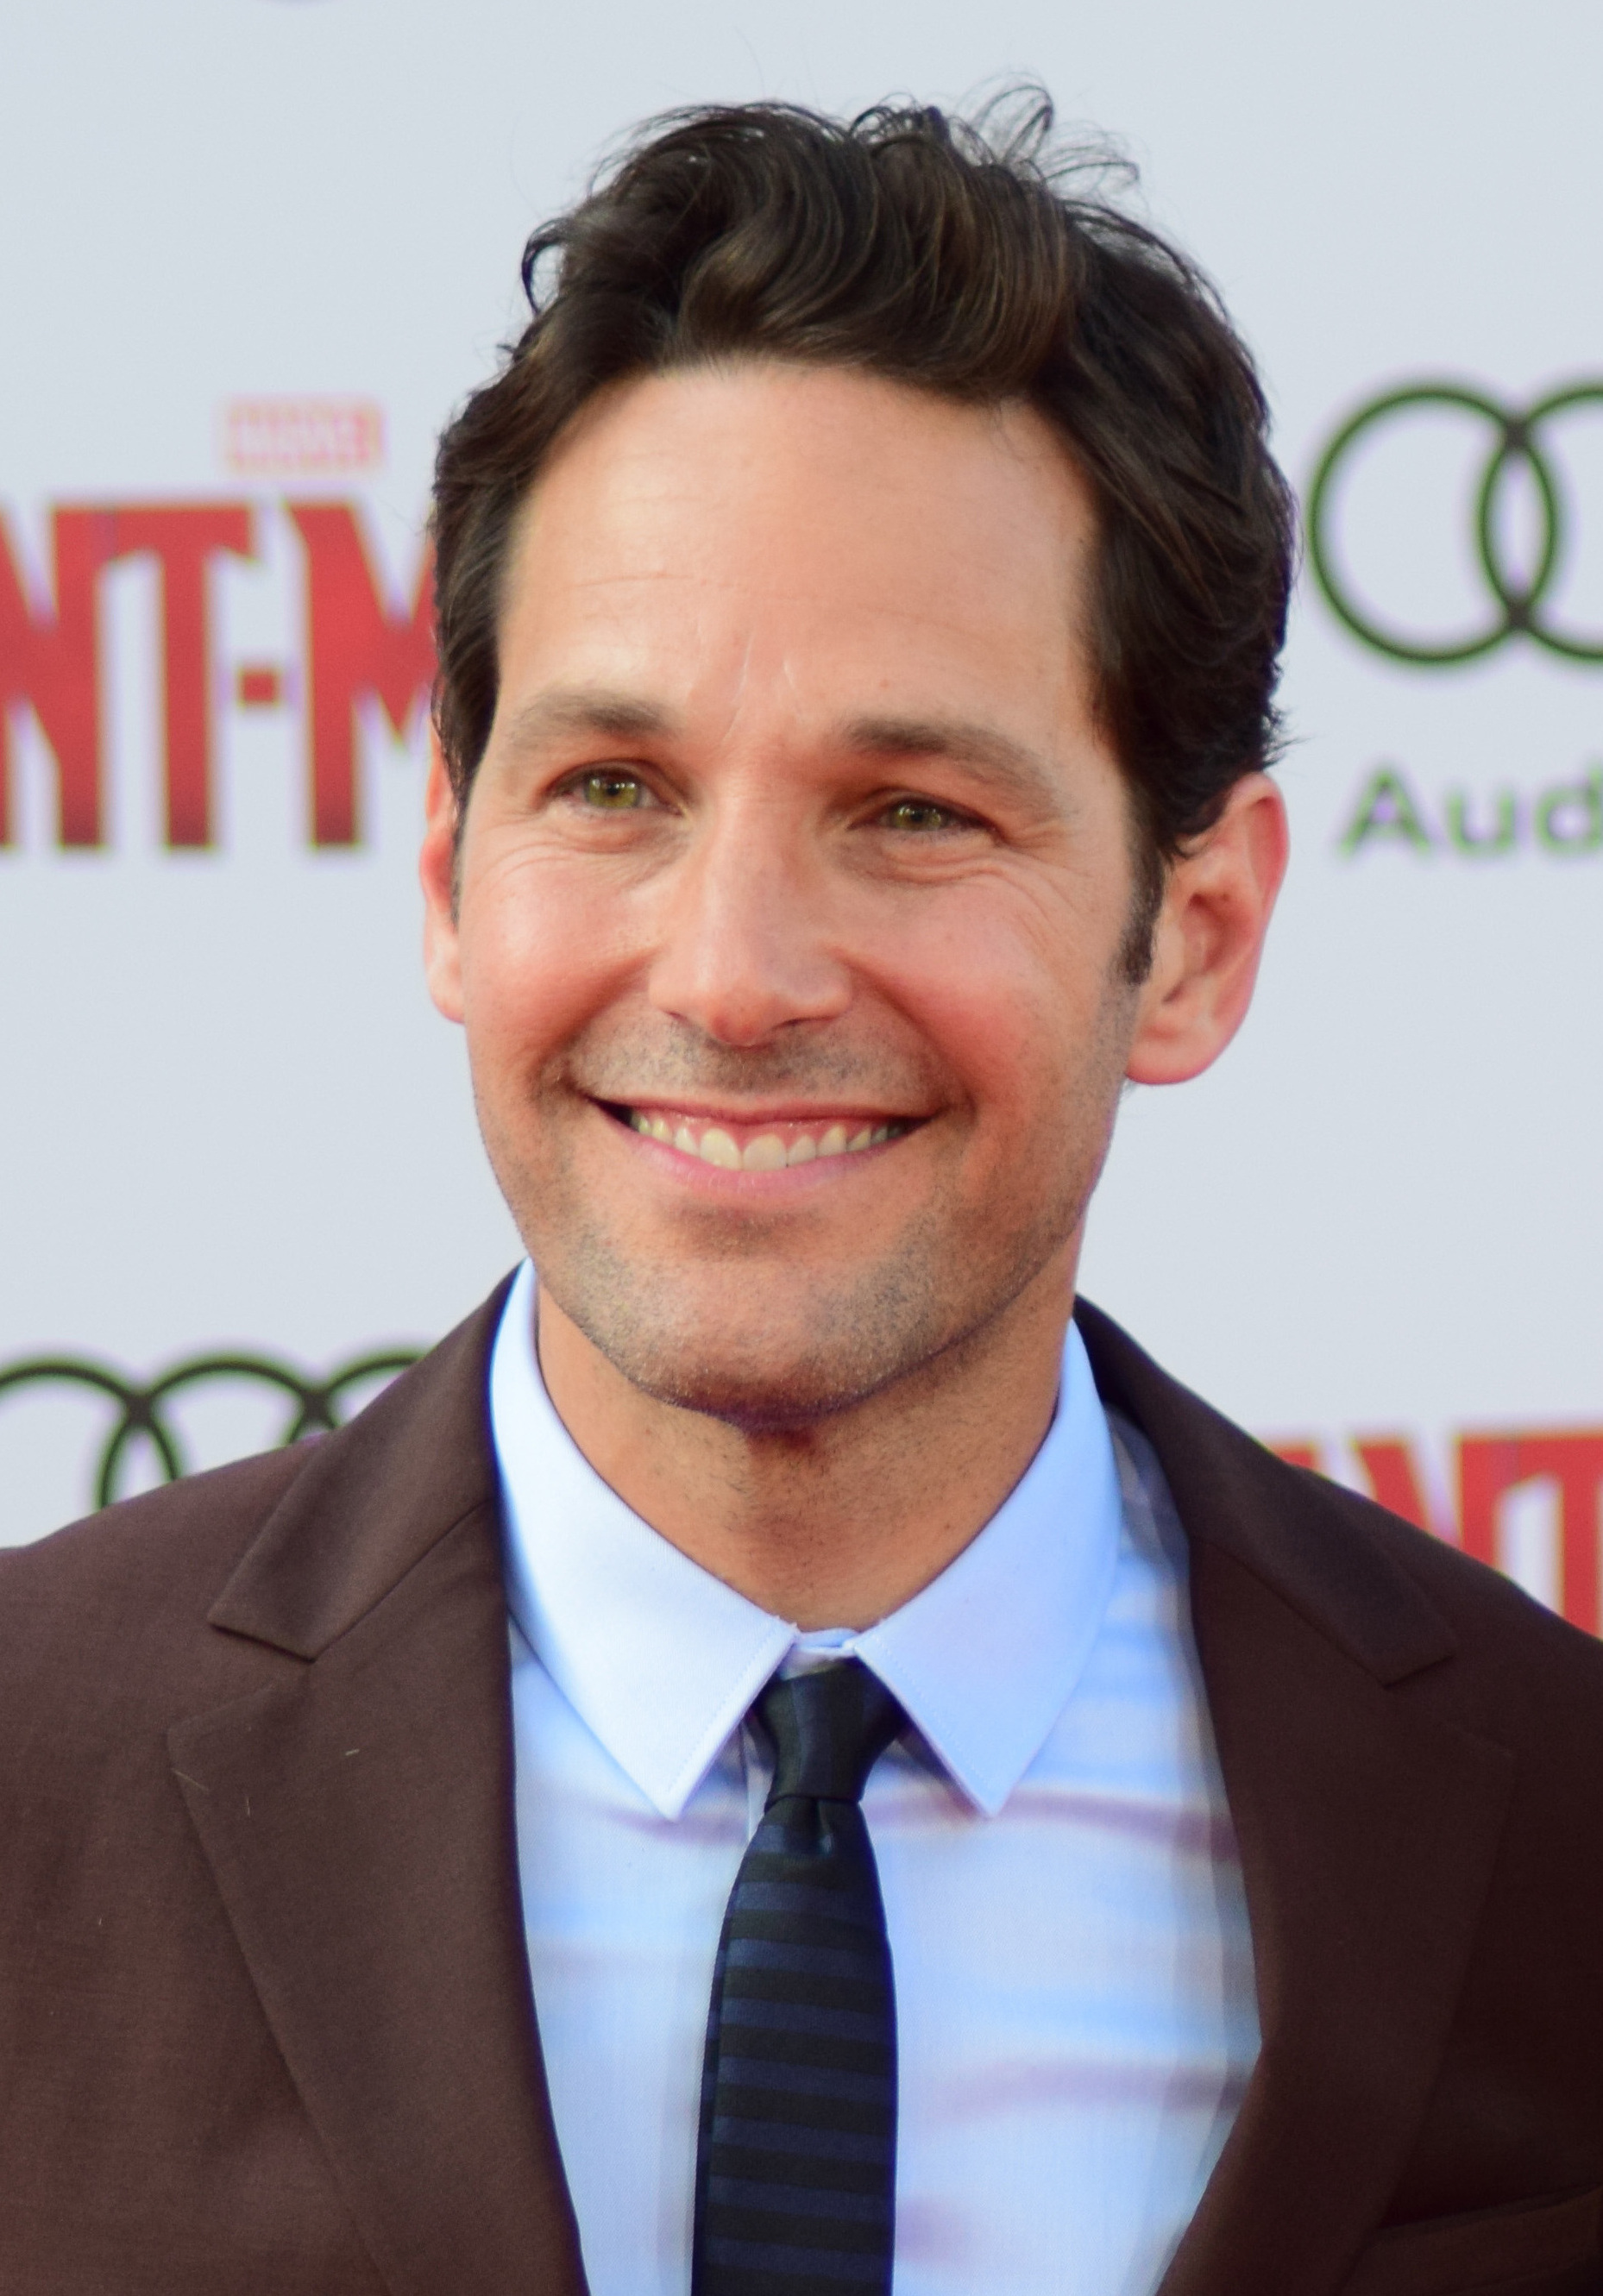
\includegraphics[scale=0.25]{paul_rudd.jpg}

      Il a quel âge? \underline{\uncover<2->{Il a 53 ans.}}
    \end{center}
  \end{frame}

  \begin{frame}{}
    \begin{center}
      \Large Quiz
    \end{center}
  \end{frame}

  \begin{frame}{Les âges de ta famille?}
    \gloss{With a partner, ask them how old different members of their family are as well as what they're like.
    For example:}
    \begin{description}
      \item[E1:] Tu as un oncle? Il a quel âge?
      \item[E2:] Mon oncle a 42 ans.
      \item[E1:] Il est comment?
      \item[E2:] Il est pessimiste et sympathique.
    \end{description}
  \end{frame}

  \begin{frame}{Des personnes idéales}
    \gloss{With a partner, use adjectives to describe your ideal version of the following. For example: \emph{Mon ami idéal est sympa et un peu indiscipliné.}}
    \begin{enumerate}
      \item ton camarade de classe ou ta camarade de classe
      \item ton professeur ou ta professeure
      \item ton ami(e)
      \item ton animal de compagnie
    \end{enumerate}
  \end{frame}

  \begin{frame}{}
    \begin{center}
      \Large Questions?
    \end{center}
  \end{frame}
\end{document}
